% !TEX root = main.tex

\section{多元函数的积分}
\subsection{重积分概述}
\begin{definition}[二重积分]
设$D$是平面上可求面积的有界闭区域,$f(x,y)$定义在$D$上,用任意曲线网将$D$分成有限个可求面积的区域$\Delta\sigma_1,\Delta\sigma_2,\ldots,\Delta\sigma_n$(称为$D$的一个分法),任取$(\xi_i,\eta_i)\in\Delta\sigma_i$,作和
\[\sigma=\sum_{i=1}^nf(\xi_i,\eta_i)\Delta\sigma_i\]
记$d_i$为$\Delta\sigma_i$的直径,$\lambda=\max_{1\leq i\leq n}\{d_i\}$,若当$\lambda\to 0$时,$\sigma$的极限存在,则称$f(x,y)$在$D$可积,并称极限值为$f(x,y)$在$D$的二重积分,记为
\[\iint_Df(P)\diff\sigma\text{或}\iint_Df(x,y)\diff x\diff y\]
也即
\[\iint_Df(x,y)\diff x\diff y=\iint_Df(P)\diff\sigma=\lim_{\lambda\to 0}\sum_{i=1}^nf(\xi_i,\eta_i)\Delta\sigma_i\]
\end{definition}
\par 二重积分的基本性质与一元定积分类似(见\ref{sub:riemann}节),在此不再赘述.
涉及可积性的证明题可能还需结合定理\ref{thm:integrality}.
\begin{example}
\begin{enumerate}
	\item 证明有界闭区域上的连续函数必可积
	\item $f$在$D$上连续,$f\geq 0$且$f\not\equiv 0$,证明$\disp\int_Df\diff D>0$
	\item 证明\[f(x,y)=\begin{cases}1 & x\in\qq\\ 0 & x\notin\qq\end{cases}\]在$[0,1]\times[0,1]$上不可积
	\item $f(x)$在$[a,b]$可积,$g(y)$在$[c,d]$可积,则$f(x)g(y)$在矩形区域$D=[a,b]\times[c,d]$可积,且
	\[\iint_Df(x)g(y)\diff x\diff y=\int_a^bf(x)\diff x\int_c^dg(y)\diff y\]
\end{enumerate}
\end{example}
\begin{analysis}
\begin{enumerate}
	\itemsep -3pt
	\item 连续函数必一致连续,则振幅可限制上界,进而对振幅与面积的乘积求和趋于$0$,可积
	\item 抽一个邻域出来,极限保号性
	\item 分别取$f(\xi_i,\eta_i)$为不同值的点,极限不同
	\item 设出$f(x),g(y)$在$\Delta\sigma_{ij}$的上下确界,分两次求和
\end{enumerate}
\end{analysis}
\begin{theorem}[富比尼(Fubini)定理]
若$f(x,y)$在矩形区域$D=[a,b]\times[c,d]$可积,且对$[a,b]$上任意$x$,含参变量积分
\[A(x)=\intabu{c}{d}{f(x,y)}{y}\]
存在,则
\[\iint_Df(x,y)\diff x\diff y=\intab{a}{b}{}\intabu{c}{d}{f(x,y)}{y}\]
即$f(x,y)$在$D$上连续,则积分次序可交换.
若$D=\{(x,y)\mid y_1(x)\leq y\leq y_2(x),a\leq x\leq b\}$,$y_1(x),y_2(x)$在$[a,b]$连续,$f(x,y)$在$D$上连续,则
\[\iint_Df(x,y)\diff x\diff y=\intab{a}{b}{}\intabu{y_2(x)}{y_1(x)}{f(x,y)}{y}\]
\end{theorem}
\par 二重积分关键确定好积分区域及积分限,有必要时注意要分段.
\par 对于三重积分的情况可以这样考虑
\begin{enumerate}
	\item 横向(平面)累加后再纵向加(注意$D_z$是变化的,即确定关于$z$的面积函数)
	\[\iiint_Vf(x,y,z)\diff x\diff y\diff z=\int_e^f\diff z\iint_{D_z}f(x,y,z)\diff x\diff y\]
	\item 纵向累加后再横向加(即投影到$D$上)
	\[\iiint_Vf(x,y,z)\diff x\diff y\diff z=\iint_D\diff x\diff y\int_{x_1(x,y)}^{x_2(x,y)}f(x,y,z)\diff z\]
\end{enumerate}
\par 由于立体空间的图像比较难想象,导致三重积分变换积分次序会比较麻烦(一共有六种情况),这时就需要逆向灵活运用上面两种方法,使三维空间的情况化归为考虑平面的情况.
\begin{example}
改变积分次序
\[I=\int_0^1\diff x\int_0^{1-x}\diff y\int_0^{x+y}f(x,y,z)\diff z\]
\end{example}
\begin{analysis}
\begin{figure}[H]
\centering
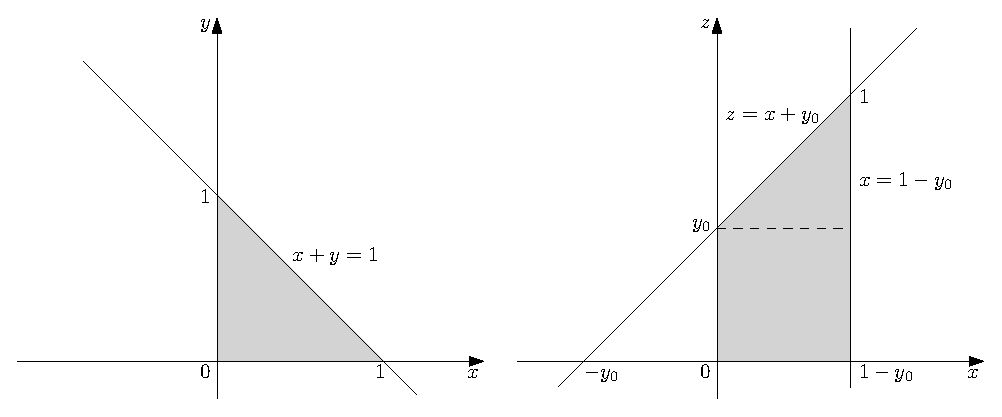
\includegraphics[width=0.6\linewidth]{fig/coordinate_eg.eps}
\end{figure}
考虑前两项,即纵向($z$方向)累加后横向加(投影到$xOy$平面上).
则可画出上图左,用二重积分的变换次序方法即可得到
\[I=\int_0^1\diff y\int_0^{1-y}\diff x\int_0^{x+y}f(x,y,z)\diff z\]
\par 再考虑后两项的次序交换,原来的后两项代表关于$x$的面积函数,则此时可以将$x$看成是常数($x_0$),这样就可以作出上图右(注意$x$的范围,以便确定直线与坐标轴交点的正负),从而又可以采用二重积分的变换方法.
注意这里需要分段求和
\[I=\int_0^1\diff y\int_0^y\diff z\int_0^{1-y}f(x,y,z)\diff x+\int_0^1\diff y\int_y^1\diff z\int_{z-y}^{1-y}f(x,y,z)\diff x\]
\par 类似地可以求得其他四种变换次序的方法.
\end{analysis}
\begin{example}
$\disp\iiint_Vxy^2z^3\diff x\diff y\diff z$,$V$由曲面$z=xy,y=x,z=0,x=1$围成
\end{example}
\begin{analysis}
对于三维空间的题目,尽可能先画出草图,确定好边界
\begin{figure}[H]
\centering
\begin{tabular}{cc}
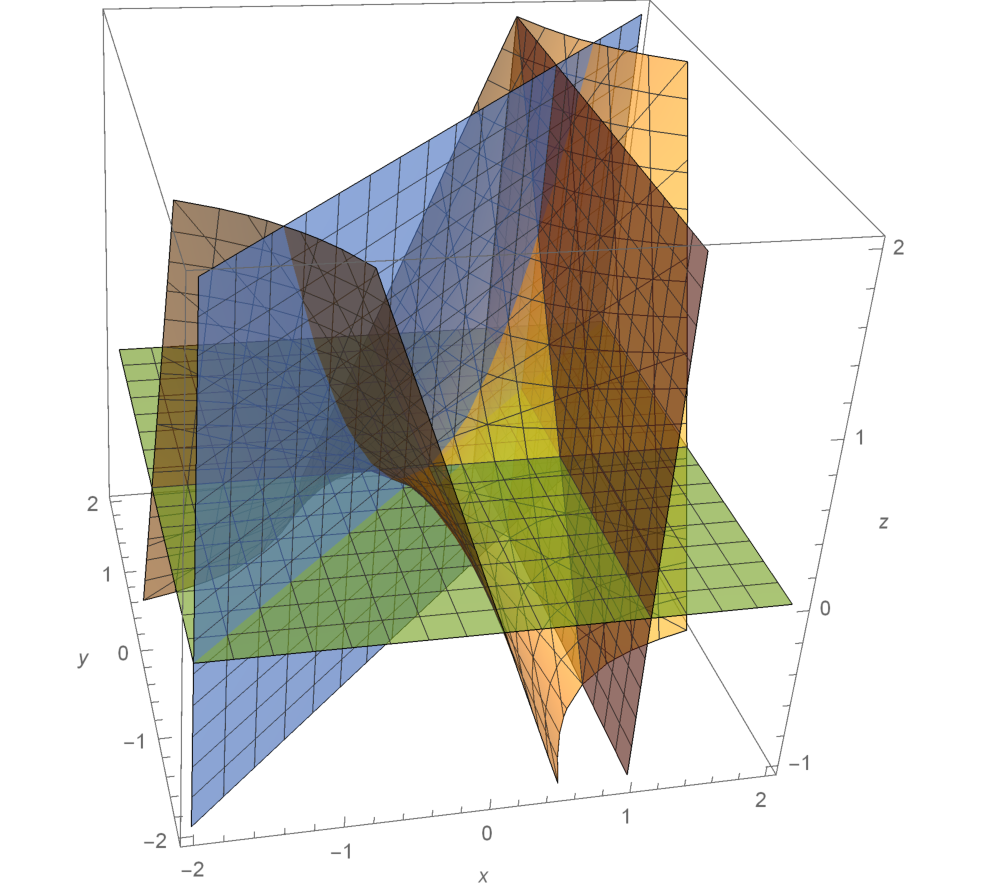
\includegraphics[width=0.4\linewidth]{fig/xy_example_side.pdf}&
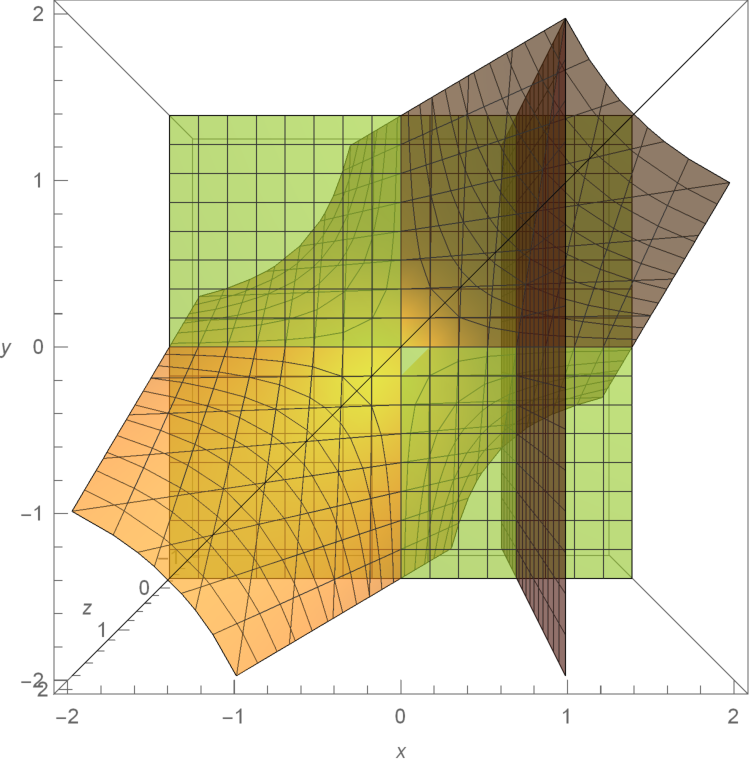
\includegraphics[width=0.3\linewidth]{fig/xy_example_front.pdf}
\end{tabular}
\end{figure}
本题中的$z=xy$形成的是一个马鞍面,在$x=0$与$y=0$两条直线上的函数值都为$0$(相当于给了一个界),且三条曲线都交于点$(1,1,1)$,进而
\[\begin{aligned}
\iiint_Vxy^2z^3\diff x\diff y\diff z&=\iint_Dxy^2\diff x\diff y\int_0^{xy}z^3\diff z\\
&=\int_0^1x\diff x\int_0^xy^2\diff y\int_0^{xy}z^3\diff z=\frac{1}{364}
\end{aligned}\]
注:此题也可出成二重积分,直接求体积($z$的两条曲线作差得到$f$)
\end{analysis}
\par 计算重积分要充分利用对称性
\begin{example}
求$\disp\iiint_V(x+y+z)\diff x\diff y\diff z,\,V:x^2+y^2+z^2\leq a^2$
\end{example}
\begin{analysis}
拆开三块进行计算,注意观察是哪项配哪项比较好算
\[\begin{aligned}
\iiint_V z\diff x\diff y\diff z&=\int_{-a}^a\diff z\iint_{D_z}z\diff x\diff y\\
&=\int_{-a}^az\diff z\iint_{D_z}\diff x\diff y\qquad\mbox{后面的二重积分直接化为面积}\\
&=\int_{-a}^az\pi(a^2-z^2)\diff z\\
&=\pi\lrp{\frac{1}{2}a^2z^2-\frac{1}{4}z^4}\Big|_{-a}^a=0
\end{aligned}\]
进而由对称性,三项均为$0$,和为$0$
\end{analysis}
\par 二重积分的几何直观是曲顶柱体的体积,或者是平面薄片的质量.
而三重积分则是四维空间曲顶柱体的体积,或者是空间物体的质量.

\subsection{重积分的变量代换}
\begin{theorem}
设变换
\[T:\begin{cases}x=\varphi(u,v)\\y=\psi(u,v)\end{cases}\]
把$Ouv$平面上由逐段光滑的闭曲线围成的区域$\Delta$一一映射为$Oxy$平面的区域$D$,且$\varphi,\psi$在$\Delta$有二阶连续偏导数,
\[J(u,v)=\frac{\partial(x,y)}{\partial(u,v)}\ne 0,\,(u,v)\in\Delta\]
而$f(x,y)$是定义在$D$上的连续函数,则
\[\iint_Df(x,y)\diff x\diff y=\iint_\Delta f(\varphi(u,v),\psi(u,v))|J(u,v)|\diff u\diff v\]
用微元的观点看,即
\[\diff S=|J(u,v)|\diff\sigma\]
注意雅可比行列式要加绝对值.
换元后$f(x,y)$会变为$f(\phi,\chi)$,而不是$f(u,v)$.
\end{theorem}
用微元的观点看会简单很多,关键确定好变换后的积分区间.
\par 三种常见的积分变换如下
\begin{enumerate}
	\item 极坐标
	\[\begin{cases}x=r\cos\theta\\y=r\sin\theta\end{cases}\implies J(r,\theta)=\frac{\partial(x,y)}{\partial(r,\theta)}=\vmat{\cos\theta & -r\sin\theta\\\sin\theta & r\cos\theta}=r\]
	\item 柱坐标变换
	\[\begin{cases}x=r\cos\theta\\y=r\sin\theta\\z=z\end{cases}\implies J(r,\theta,z)=\frac{\partial(x,y,z)}{\partial(r,\theta,z)}=\vmat{\cos\theta & -r\sin\theta & 0\\\sin\theta & r\cos\theta & 0\\ 0 & 0 & 1}=r\]
	\item 球坐标变换
	\begin{figure}[H]
	\centering
	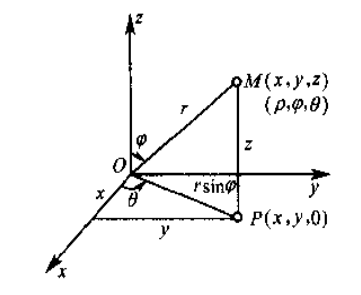
\includegraphics[width=0.3\linewidth]{fig/ball_coordinate.PNG}
	\end{figure}
	\[\begin{cases}x=r\sin\varphi\cos\theta&0\leq r<+\infty\\y=r\sin\varphi\sin\theta&0\leq\theta<2\pi\\z=r\cos\varphi & 0\leq\varphi\leq\pi\end{cases}\implies J(r,\theta,\varphi)=\vmat{\cos\theta\sin\varphi & -r\sin\theta\sin\varphi & r\cos\theta\cos\varphi\\\sin\theta\sin\varphi & r\cos\theta\sin\varphi & r\sin\theta\cos\varphi\\ \cos\varphi & 0 & -r\sin\varphi}=-r^2\sin\varphi\]
\end{enumerate}
\par 变换的目的是好算,最好变换成长方形区域,故要观察特征,抽取相同项出来,如下例.
\begin{example}
\begin{itemize}
	\item $D$由$y=4x^2,y=9x^2,x=4y^2,x=9y^2$围成
	\[T^{-1}:\;y^2=ux,x^2=vy\implies u=\frac{y^2}{x},v=\frac{x^2}{y}\]
	\item $D$由$xy=2,xy=4,y=x,y=2x$围成
	\[T^{-1}:\;u=xy,y=vx\implies u=xy,v=\frac{y}{x}\]
\end{itemize}
\end{example}

\subsection{含参变量正常积分}
含参变量积分其实就对应着概率论里面的边缘概率密度,而二重积分则是联合概率密度.
\begin{theorem}
对于含参变量积分$I(x)=\disp\int_c^df(x,y)\diff y$,$f(x,y)$在$[a,b]\times [c,d]$上连续,有
\begin{enumerate}
	\item 积分与极限互换:$I(x)$在$[a,b]$连续
	\item 积分与导数互换:$f_x$也在$[a,b]\times [c,d]$连续,则$I(x)$在$[a,b]$有连续导函数
	\[I'(x)=\int_c^df_x(x,y)\diff y\]
	\item 积分交换次序:
	\[\intab{a}{b}{}\intabu{c}{d}{f(x,y)}{y}=\intabu{c}{d}{}{y}\intab{a}{b}{f(x,y)}\]
\end{enumerate}
(对于变上限积分$I(x,u)=\disp\int_c^uf(x,y)\diff y$也是一样)
\end{theorem}
\par 将下式称为先对$y$后对$x$的累次积分
\[\int_a^bI(x)\diff x=\int_a^b\left[\int_c^df(x,y)\diff y\right]\diff x=\intab{a}{b}{}\intabu{c}{d}{f(x,y)}{y}\]
\begin{example}
$\disp I(a)=\int_0^\pi\ln(1-2a\cos x+a^2)\diff x,\,|a|<1$
\end{example}
\begin{analysis}
$f(a,x)=\ln(1-2a\cos x+a^2),\,f_a(a,x)=\dfrac{2a^2-2a\cos x}{1-2a\cos x+a^2}$,由$\Delta=4\cos^2x-4<0$知$1-2a\cos x+a^2>0$恒成立,进而$f(a,x)$与$f_a(a,x)$都在$[-1,1]$连续,$I(a)$在积分号下可求导数
\[\begin{aligned}
I'(a)&=\intab{0}{\pi}{f_a(a,x)}\\
&=\frac{1}{a}\intab{0}{\pi}{\frac{2a^2-2a\cos x}{1-2a\cos x+a^2}}\\
&=\frac{1}{a}\intab{0}{\pi}{1+\frac{a^2-1}{1-2a\cos x+a^2}}\qquad\mbox{把分子的$\cos$项消去}\\
&=\frac{x}{a}\Big|_0^\pi+\frac{a^2-1}{a}\intab{0}{+\infty}{\frac{1}{a^2-2a\cos x+1}}\\
&=\frac{\pi}{a}+\frac{a^2-1}{a}\int_0^{+\infty}\frac{\frac{2}{1+t^2}\diff t}{a^2-2a\frac{1-t^2}{1+t^2}+1}\qquad\mbox{令}t=\tan\frac{x}{2}\in[0,+\infty),\text{即}x=2\arctan t\\
&=\frac{\pi}{a}+2\frac{a^2-1}{a}\int_0^{+\infty}\frac{\diff t}{t^2(a+1)^2+(a-1)^2}\\
&=\frac{\pi}{a}+2\frac{a^2-1}{a}\frac{1}{(a-1)^2}\int_0^{+\infty}\frac{\diff t}{1+\lrp{\frac{a+1}{a-1}t}^2}\\
&=\frac{\pi}{a}+\frac{2}{a}\arctan\lrp{\frac{a+1}{a-1}t}\Big|_0^{+\infty}\qquad|a|<1,\frac{a+1}{a-1}\mbox{为负数}\\
&=\frac{\pi}{a}-\frac{2}{a}\cdot\frac{\pi}{2}=0
\end{aligned}\]
故$I(a)=\disp\int 0\diff a=0$\\
另外,
\begin{itemize}
	\itemsep -3pt
	\item 对于一般的情况还需解出常数$C$
	\item 本题还可联系例\ref{eg:sum_fun_analysis}
	\item 对于$a\geq 0$的其他情况,可见\footnote{\url{https://math.stackexchange.com/questions/650513/computing-int-0-pi-ln-left1-2a-cos-xa2-right-dx}}
\end{itemize}
\end{analysis}
\begin{theorem}
设函数$f(x,y)$在$[a,b]\times[c,d]$上连续,
\begin{enumerate}
	\item $c(x),d(x)$都在$[a,b]$上连续,并且当$x\in[a,b]$时,有$c\leq c(x),d(x)\leq d$,则
	\[F(x)=\int_{c(x)}^{d(x)}f(x,y)\diff y\]
	在$[a,b]$连续
	\item $f_x$也在$[a,b]\times[c,d]$连续,又$c'(x)$和$d'(x)$在$[a,b]$存在,则变上限积分$F(x)$可导,且
	\[F'(x)=\int_{c(x)}^{d(x)}f_x(x,y)\diff y+f(x,d(x))d'(x)-f(x,c(x))c'(x)\]
\end{enumerate}
\end{theorem}

\subsection{含参变量的广义积分}
\label{sec:sub:parameter_abnormal_integral}
\begin{definition}[一致收敛]
设$f(x,y)$定义在$[a,b]\times[c,+\infty)$,且对任意$x\in[a,b]$,无穷积分
\[I(x)=\int_c^{+\infty}f(x,y)\diff y\]
收敛.
若
\[\forall x\in[a,b],\eps>0\exists A_0>c, A>A_0:\;\left|\int_c^Af(x,y)\diff y-I(x)\right|<\eps\quad\text{或}\quad\left|\int_A^{+\infty}f(x,y)\diff y\right|<\eps\]
则称广义积分$I(x)$在$[a,b]$一致收敛.\\
定义中的区间可换为开区间、半开半闭区间等.
\end{definition}
\begin{theorem}[M判别法(Weierstrass)]
若存在$M(y)$使得与常数$B>c$,
\[|f(x,y)|\leq M(y),\forall y\geq B,x\in[a,b]\]
而广义积分$\disp\int_c^{+\infty}M(y)\diff y$收敛,则$\intabu{c}{+\infty}{f(x,y)}{y}$在$[a,b]$一致收敛
\end{theorem}
\begin{theorem}[迪尼(Dini)]
设$f(x,y)$在$[a,+\infty)\times[c,d]$连续且非负.
若$\intab{a}{+\infty}{f(x,y)}$在$[c,d]$收敛,且作为$y$的函数在$[c,d]$连续,则$\intab{a}{+\infty}{f(x,y)}$在$[c,d]$一致收敛
\end{theorem}
\par 关于一致收敛的其他定理,可见\ref{summary_conver}节,只需注意所有的定理条件都是对于积分变量而言的.
如狄利克雷判别法中$g(x,y)$关于积分变量$y$单调一致趋于$0$;阿贝尔判别法中$g(x,y)$关于积分变量$y$单调有界($y\geq$积分下限).
\par 类比定理\ref{thm:sum_function_analysis_properties},有以下性质.
\begin{theorem}
对于含参变量广义积分$\disp I(x)=\int_c^{+\infty}f(x,y)\diff y$,$f(x,y)$在$[a,b]\times [c,+\infty)$上连续,
\begin{enumerate}
	\item 积分与极限互换:若$I(x)$在$[a,b]$一致收敛,则$I(x)$在$[a,b]$连续
	\item 积分与导数互换:$f_x$也在$[a,b]\times [c,d]$连续,若$\disp\intabu{c}{+\infty}{f(x,y)}{y}$在$[a,b]$收敛,$\disp\intabu{c}{+\infty}{f_x(x,y)}{y}$在$[a,b]$一致收敛,则$I(x)$在$[a,b]$可导,且
	\[I'(x)=\int_c^{+\infty}f_x(x,y)\diff y\]
	\item 积分交换次序:若$I(x)$在$[a,b]$一致收敛,则
	\[\intab{a}{b}{}\intabu{c}{d}{f(x,y)}{y}=\intabu{c}{d}{}{y}\intab{a}{b}{f(x,y)}\]
\end{enumerate}
\end{theorem}
\begin{example}
求狄利克雷积分$I=\intab{0}{+\infty}{\frac{\sin x}{x}}$
\end{example}
\begin{analysis}
\begin{itemize}
\item 引入因子$\ee^{-xy}(y\geq 0)$使其变为含参变量积分
\[I(y)=\intab{0}{+\infty}{\ee^{-xy}\frac{\sin x}{x}}\]
\item 因为$\intab{0}{+\infty}{\frac{\sin x}{x}}$收敛(狄利克雷),又对每一个$y\in[0,+\infty)$,函数$\ee^{-xy}$关于$x$是单调函数,且
\[|\ee^{-xy}|\leq 1,\,x,y\in[0,+\infty)\]
由阿贝尔判别法,$\intab{0}{+\infty}{f(x,y)}$在$[0,+\infty)$一致收敛.
\item 由上式一致收敛及$f(x,y)=\ee^{-xy}\dfrac{\sin x}{x}$在$[0,+\infty)\times[0,+\infty)$连续,故积分与极限可互换,从而$I=I(0)=\disp\lim_{y\to 0^+}I(y)$
\item 为求$I(y)$,先求$I'(y)$.
由构造式有$f_y(x,y)=-\ee^{-xy}\sin x$,
\[\forall a>0:\;|f_y(x,y)|=|\ee^{-xy}\sin x|\leq \ee^{-ax},\,y\geq a>0\]
而$\intab{0}{+\infty}{\ee^{-ax}}$收敛,由M判别法,$\intab{0}{+\infty}{f_y(x,y)}$在$[a,+\infty)$一致收敛
\item 又$f_y(x,y)$在$[0,+\infty)\times[0,\infty)$连续,故积分与导数可互换,即$I(y)$在$[a,+\infty)$可导,且
\[I'(y)=\intab{0}{+\infty}{f_y(x,y)}=-\intab{0}{+\infty}{\ee^{-xy}\sin x}=\frac{-1}{1+y^2},\,y>0\]
故$I(y)=\disp\int\frac{-1}{1+y^2}=-\arctan y+C$
\item 注意到$\dfrac{\sin x}{x}$在$[0,+\infty)$有界,故$y>0$时,
\[\intab{0}{+\infty}{\ee^{-xy}\frac{\sin x}{x}}\leq M\intab{0}{+\infty}{\ee^{-xy}}=\frac{M}{y}\]
即当$y\to +\infty$时,左侧积分为$0$.
故$\disp c=\lim_{y\to\infty}\arctan y=\frac{\pi}{2}$,有$I(y)=-\arctan y+\frac{\pi}{2}$,进而
\[I=I(0)=\lim_{y\to 0^+}I(y)=\frac{\pi}{2}\]
\end{itemize}
注:本题进一步可得
\[\intab{0}{+\infty}{\frac{\sin\alpha x}{x}}=\frac{\pi}{2}\sgn\alpha\]
\end{analysis}
\begin{theorem}
设$f(x,y)$在$[a,+\infty)\times[c,+\infty)$连续且非负,
\[\intab{a}{+\infty}{f(x,y)},\intabu{c}{+\infty}{f(x,y)}{y}\]
都收敛,且分别在$[c,+\infty)$和$[a,+\infty)$连续,则(若存在)
\[\int_c^{+\infty}\diff y\intab{a}{+\infty}{f(x,y)}=\int_a^{+\infty}\diff x\intabu{c}{+\infty}{f(x,y)}{y}\]
\end{theorem}

\subsection{欧拉积分}
\subsubsection{第二欧拉积分}
\[\Gamma(\alpha)=\intab{0}{+\infty}{x^{\alpha-1}\ee^{-x}},\,\alpha>0\]
分析性质:
\begin{enumerate}
	\item 在定义域$\alpha>0$内连续且有任意阶连续导数
	\[\Gamma^{(n)}(\alpha)=\intab{0}{+\infty}{x^{\alpha-1}(\ln x)^n\ee^{-x}}\]
	\item 递推公式
	\[\Gamma(\alpha+1)=\alpha\Gamma(\alpha)\]
	特别地,当$\alpha\in\zz^+$时
	\[\Gamma(\alpha+1)=\alpha!\]
	对于任意$\alpha>0$,总存在非负整数$n$使得$\alpha=n+p,\,p\in(0,1]$,则
	\[\Gamma(\alpha)=\Gamma(n+p=(n+p-1)\cdots(1+p)p\Gamma(p)\]
	\item $\Gamma(1)=1$;由概率积分可得$\Gamma(\frac{1}{2})=\sqrt{\pi}$
\end{enumerate}
概率分布中会用到的其他公式
\begin{itemize}
\item 上不完全(upper incomplete)伽马函数
\[ \Gamma(s,x) = \int_x^{\infty} t^{s-1}\ee^{-t}\diff t\]
\item 下不完全(lower incomplete)伽马函数
\[ \gamma(s,x) = \int_{0}^{x}t^{s-1}\ee^{-t}\diff t\]
\item 递推关系
\[\begin{aligned}
\Gamma(s,x)&=(s-1)\Gamma(s-1,x) + x^{s-1} \ee^{-x}\\
\gamma(s,x)&=(s-1)\gamma(s-1,x) - x^{s-1} \ee^{-x}\\
\Gamma(s) &= \Gamma(s,0)\\
\gamma (s,x)&+\Gamma (s,x)=\Gamma (s)
\end{aligned}\]
\end{itemize}

\subsubsection{第一欧拉积分}
\[B(a,b)=\intab{0}{1}{x^{a-1}(1-x)^{b-1}},\,a,b>0\]
分析性质:
\begin{enumerate}
	\item 对称性:$B(a,b)=B(b,a)$
	\item 递推公式
	\[\begin{aligned}
	B(a,b)&=\frac{b-1}{a+b-1}B(a,b-1),\,a>0,b>1\\
	&=\frac{a-1}{a+b-1}B(a-1,b),\,a>1,b>0
	\end{aligned}\]
	\item 狄利克雷公式
	\[B(a,b)=\frac{\Gamma(a)\Gamma(b)}{\Gamma(a+b)},\,a>0,b>0\]
\end{enumerate}